% Figure s01f04_cdw (Session 1): the charge density wave of the spinless chain, in real space and in the spectrum.
% The image is rendered by figures/blender/s01f04_cdw.py; the coordinates of the labels come from
% figures/blender/out/s01f04_cdw_anchors.tex. Build with figures/blender/build_figure.sh s01f04_cdw.
\documentclass[11pt,tikz,border=0pt]{standalone}
\usepackage[T1]{fontenc}
\usepackage{amsmath,amssymb,graphicx}
\usepackage{xcolor}
\usetikzlibrary{arrows.meta}
% The three label colors of the figures, with the same values as in src/figures_preamble.tex.
\definecolor{aqmaccent}{RGB}{31,78,121}
\definecolor{aqmbroken}{RGB}{168,42,34}
\definecolor{aqmmuted}{RGB}{125,125,125}

\newlength{\figw}\setlength{\figw}{15.6cm}   % the text width of the notes (A4, 2.7 cm margins)

\begin{document}
\begin{tikzpicture}[lbl/.style={font=\small, inner sep=1.5pt},
    flow/.style={line width=0.9pt, -{Stealth[length=5pt,width=4pt]}}]
  \node[anchor=south west, inner sep=0pt] at (0,0)
    {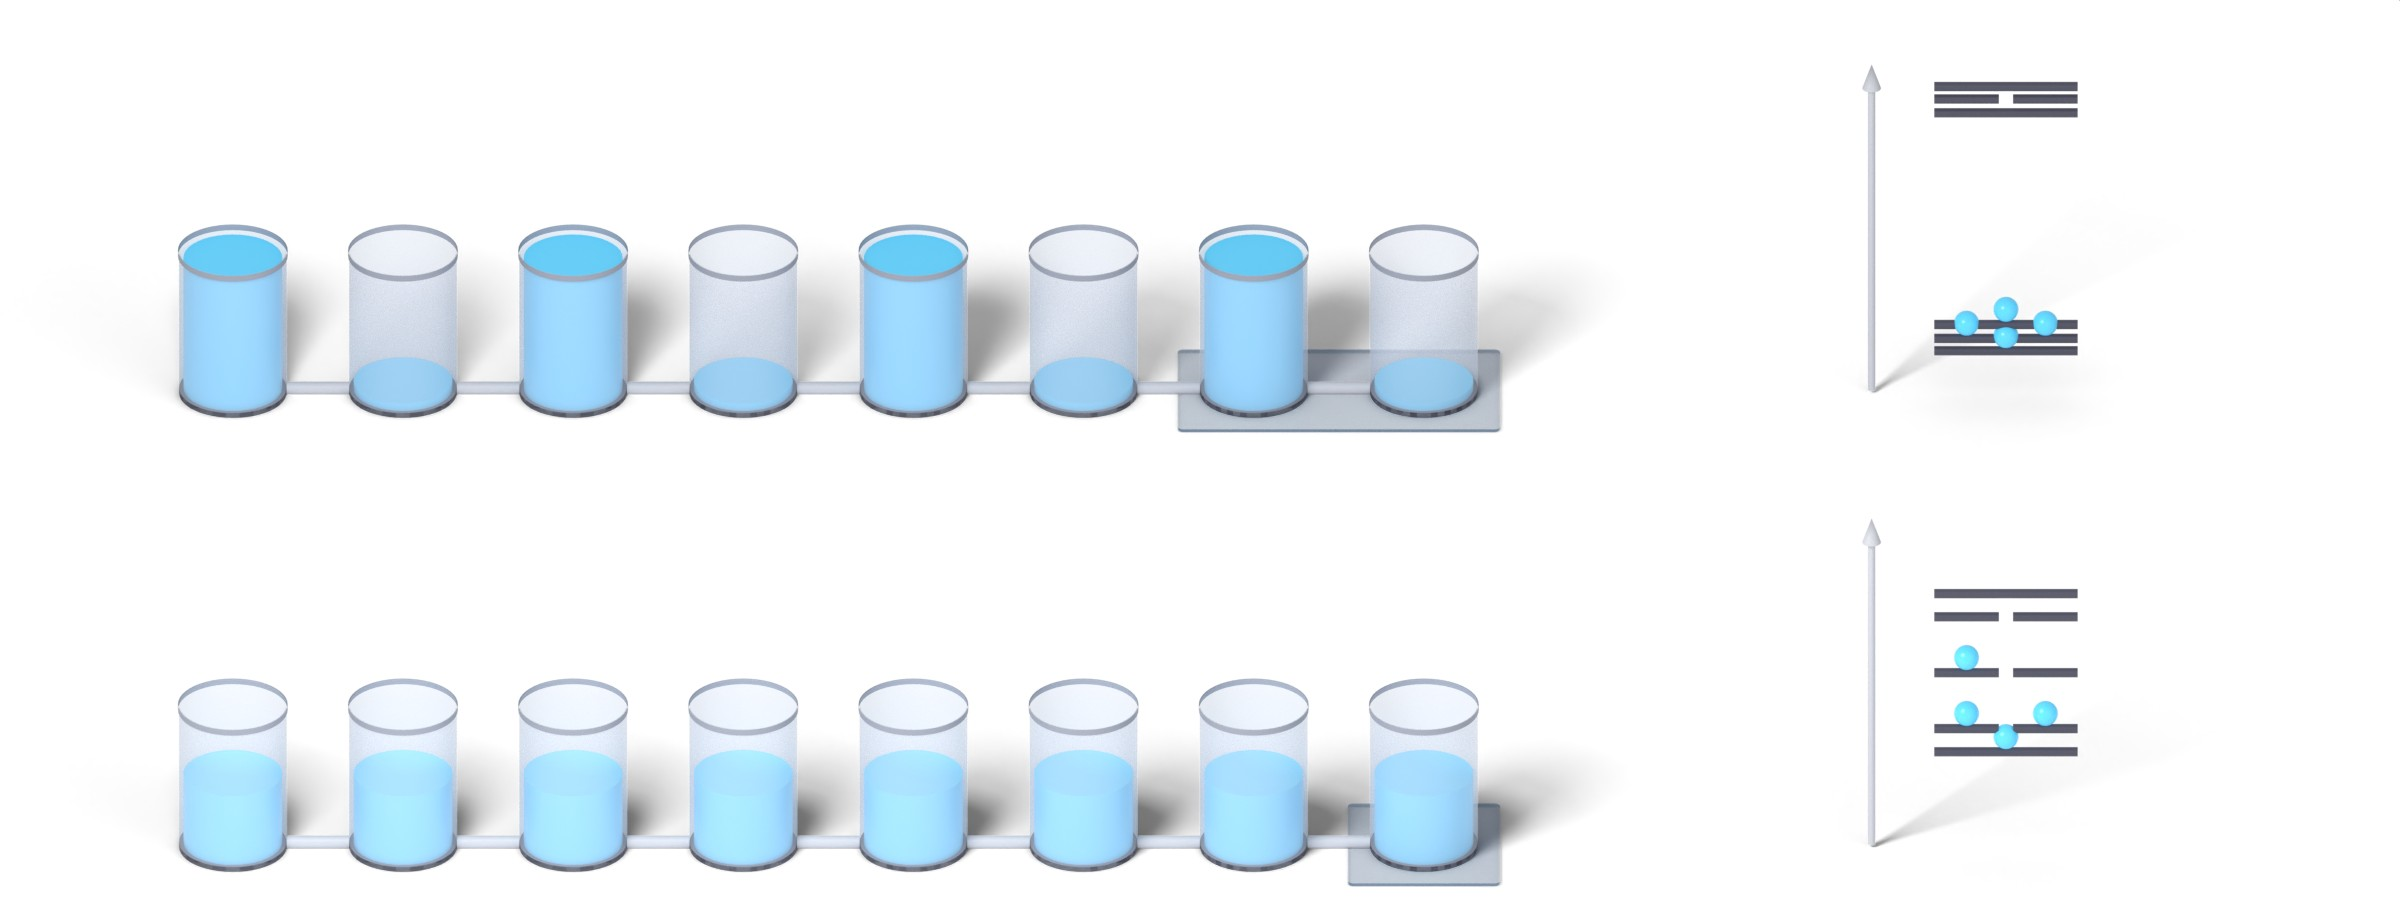
\includegraphics[width=\figw]{../blender/out/s01f04_cdw.jpg}};
  %% written by figlib.py; x and y in units of the image width
\coordinate (acell) at (0.6269\figw,0.0318\figw);
\coordinate (aE) at (0.7799\figw,0.1718\figw);
\coordinate (aspec) at (0.8731\figw,0.1043\figw);
\coordinate (apanel) at (0.0634\figw,0.1208\figw);
\coordinate (bcell) at (0.6269\figw,0.2210\figw);
\coordinate (bE) at (0.7799\figw,0.3610\figw);
\coordinate (bspec) at (0.8731\figw,0.2935\figw);
\coordinate (bpanel) at (0.0634\figw,0.3099\figw);

  \node[lbl, anchor=south west] at (apanel) {$V=0$, $\langle n_i\rangle=\tfrac12$ on every site};
  \node[lbl, anchor=south west, text=aqmbroken] at (bpanel) {$V=3t$, $\langle n_i\rangle=0.95,\,0.05,\,0.95,\dots$};
  \node[lbl, anchor=west, text=aqmmuted] at (acell) {unit cell $a$};
  \node[lbl, anchor=west, text=aqmmuted] at (bcell) {unit cell $2a$};
  \node[lbl, anchor=south] at (aE) {$E$};
  \node[lbl, anchor=south] at (bE) {$E$};
  \node[lbl, anchor=west] at (aspec) {gapless};
  \node[lbl, anchor=west, text=aqmbroken] at (bspec) {gap};
\end{tikzpicture}
\end{document}
